\subsection*{Измерения}

\textbf{Измерения спектра}.
Измерим гамма-спектр для \na, \cs, \co, \am, и \eu (см. дополнение, общий вид спектра). Измерим фон (рис. \ref{fig:background}). Все измерения проводились в течение $\tau = $ 10 минут. Погрешность соответствующего измерения можем найти, как
\begin{equation*}
    \eta(n) = \frac{N }{\tau}\pm \frac{\sqrt{N}}{\tau},
    \hspace{10 mm} 
    \eta - \eta_0 = 
    \frac{N-N_0}{\tau}\pm \frac{\sqrt{N}+\sqrt{N_0}}{\tau}.
\end{equation*}
где $n$ -- номер канала, $N$ -- количество зарегистрированных частиц, $\eta = N/\tau$ -- количество частиц в секунду, $\eta_0$ -- фоновый спектр.


\textbf{Аппроксимация}.
Аппроксимируем соответствующие части спектра гауссом $+$ полином (степень указана в подписи к соответствующему графику). Далее $\mu$ -- номер канала, соответствующего максимуму гауссианы, $\sigma$ -- среднеквадратичное отклонение.

В силу маленького значения $\Delta(\mu)$, но наличия чувствительности к аппроксимирующей функции погрешность измерения максимума далее считается равной 1 каналу: $\Delta(\mu) \equiv 1$. 


\textbf{Калибровка}.
В частности, для калибровки важны значения пиков полного поглощения для \na и \cs:
\begin{equation*}
    \mu(\text{\na})_1 = 739,
    \hspace{5 mm} 
    \mu(\text{\na})_2 = 1823,
    \hspace{10 mm} 
    \mu(\text{\cs}) = 952,
\end{equation*}
которым соответствуют значения энергии в 511 кэВ, 662 кэВ, 1275 кэВ, соответственно.

По трём значениям найдём калибровочную функцию $E(n) = a_c n + b_n$, см.  рис. \ref{fig:сalibr}.
\begin{figure}[h]
    \centering
    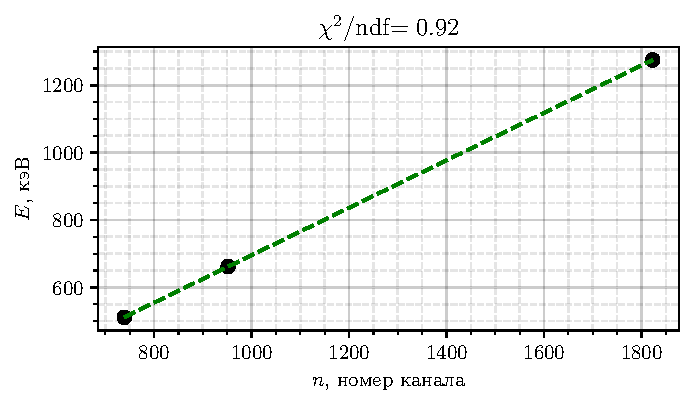
\includegraphics[width=0.5\textwidth]{figures/calibr.pdf}
    \caption{Калибровка спектрометра}
    \label{fig:сalibr}
\end{figure}
И, соответственно, параметры $E(n)$:
\begin{equation*}
    % \cov = \begin{pmatrix}
    %     7 \cdot 10^{-7} & -8 \cdot 10^{-4}  \\
    %     -8 \cdot 10^{-4} &  1.1 \\
    % \end{pmatrix},
    % \hspace{10 mm} 
    a_c = (0.705 \pm 0.001) \text{ кэВ},
    \hspace{10 mm} 
    b_c = (-9 \pm 1) \text{ кэВ}.
\end{equation*}
Погрешность соответствующего перехода $n \to E$ можно оценить, как
\begin{equation*}
    \Delta[E(n)] = 
    \left[(1,\, n)
              \cov 
              (1,\, n)\T
               + (\Delta(\mu) \cdot a_c)^2\right]^{1/2}
               =
               \left[(1,\, n)
              \cov 
              (1,\, n)\T
               + a_c^2\right]^{1/2}
               .
\end{equation*}



\textbf{Фотопики}. Зная калибровку, находим соответствующие максимумы $\mu_i (n_i)$ (см. дополнение, параметры аппроксимации), и находим соответствующие значения энергии $\sub{E}{fa}$:
\begin{align*}
    % \sub{E}{fa}(\text{\na}) &= \{\} \text{ кэВ}, \\  
    % \sub{E}{fa}(\text{\cs}) &= \{\} \text{ кэВ}, \\ 
    \sub{E}{fa}(\text{\co}) &= \{1174 \pm 2, 1334 \pm 2\} \text{ кэВ}, \\ 
    \sub{E}{fa}(\text{\am}) &= \{62 \pm 2\} \text{ кэВ}, \\ 
    \sub{E}{fa}(\text{\eu}) &= \{125 \pm 2, 245 \pm 2, 343 \pm 1\} \text{ кэВ},
\end{align*}
что, например, сходится с табличным значением для \co:
\begin{equation*}
    \sub{E}{fa}^{\text{table}}(\text{\co}) = \{1173, 1332\} \text{ кэВ}.
\end{equation*}


\newpage 

\textbf{Разрешение спектрометра}. Для проверки формулы 1, из аппроксимации определим ширины (полная ширина на полувысоте) соответствующих пиков:
\begin{equation*}
    \delta E_i = \text{FWHM} = 2 \sqrt{2 \ln 2} \sigma_i \times a_c,
\end{equation*}
где соответствующие $\sigma_i$ указаны в дополнение. 

Построим $R^2(1/E)$, и аппроксимируем линейной зависимостью $R^2 = a_R/E + b_R$.
\begin{figure}[h]
    \centering
    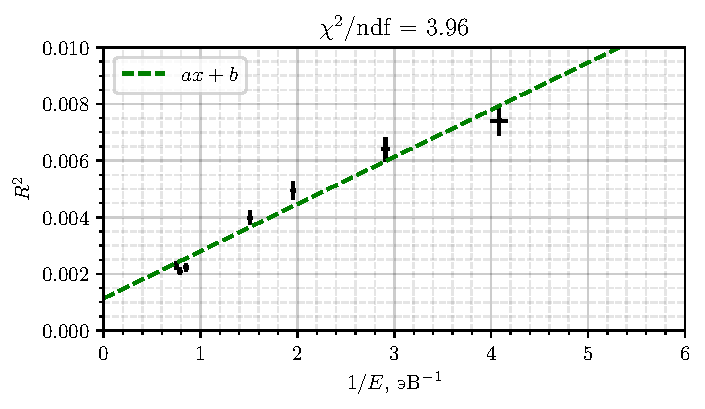
\includegraphics[width=0.6\textwidth]{figures/dpi.pdf}
    \caption{Проверка зависимости для разрешения спектрометра $R^2 \sim 1/E$}
    %\label{fig:}
\end{figure}
Видно, что при достаточно больших энергиях формула (1) прекрасно выполняется, так, например при аппроксимации прямой вплоть до $E = 244$ кэВ, $\xi^2/$ndf составило 4.0. Погрешности обусловлены погрешностью $a_c$, $\sigma_i$, функции $E(n_i)$ и $\Delta \mu$.



\textbf{Пики обратного рассеяния}. Аналогично, аппроксимируем пики обратного рассеяния для исследуемых веществ (см. дополнение), что определить соответствующие $n_i$. 



\begin{figure}[h]
    \centering
    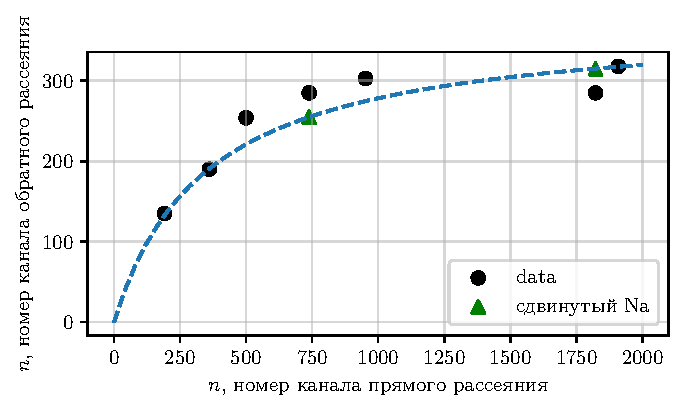
\includegraphics[width=0.6\textwidth]{figures/back.pdf}
    \caption{Сравнение наблюдаемых пиков обратного рассеяния с теоретическими значениями}
    \label{fig:3}
\end{figure}

Заметим, что для \na два пика обратного рассеяния неразличимы, однако они отстоят от теоретической кривой на равное расстояние. Сдвинутые на равные значения $n_i^{\text{эксп}}$ для \na  отображены треуголными маркерами, пунктирной линией построена зависимость (2).

Видно, что наблюдаемые пики обратного рассеяния находятся близко к теоретической кривой. 


\newpage 

\textbf{Комптоновское рассеяние}. Также определим по снятому спектру край спектра $\sub{E}{к}$ комптоновских электронов. Для этого по экспериментальным данным строился сплайн, 1/2 от начала явного спада считалась границей. 
В силу условности границы, погрешностью считалась 1/4 от размеров спада. 
Так приходим к значениям 
\begin{align*}
    \sub{E}{к}(\text{\na}) &= \{336 \pm 5,\, 1048 \pm 18\} \text{ кэВ}, \\  
    \sub{E}{к}(\text{\cs}) &= \{469 \pm 10\} \text{ кэВ}, \\ 
    \sub{E}{к}(\text{\co}) &= \{956 \pm 18\} \text{ кэВ}, \\ 
    \sub{E}{к}(\text{\am}) &= \{32 \pm 1\} \text{ кэВ},
\end{align*}
что в пределах погрещности совпадает с табличными значениями
\begin{align*}
    \sub{E}{к}^{\text{table}}(\text{\na}) &= \{341,\, 1062\} \text{ кэВ}, \\  
    \sub{E}{к}^{\text{table}}(\text{\cs}) &= \{477\} \text{ кэВ}, \\ 
    \sub{E}{к}^{\text{table}}(\text{\co}) &= \{960\} \text{ кэВ}.
\end{align*}